\section{The fragments $\AAbarBBbarEbar$ and $\AAbarEBbarEbar$: ex\-po\-nen\-tial small-model property}\label{sec:AAbarBBbarEbar}

Before going into the details of the section, we would like to summarize the main ideas of~\cite{MMP15},
in which the authors gave the first exponential small-model for $\AAbarBBbarEbar$ and $\AAbarEBbarEbar$, different from the one we shall see in the following.

We recall from Chapter~\ref{chap:MCfullHShomo} that
being associated with the same $B$-descriptor is a sufficient condition for two traces to be indistinguishable with respect to the fulfillment of $\AAbarBBbarEbar$ formulas, provided that the B-nesting depth of the considered formula is less than or equal to the depth of the descriptor itself. 
Thus we may say that a $B_k$-descriptor provides a finite encoding for a possibly infinite set of traces (the traces associated with that descriptor). Unfortunately, the representation of $B_k$-descriptors as trees labelled over descriptor elements is highly redundant. For instance, given any pair of subtrees rooted in some children of the root of a descriptor, it is always the case that one of them is a subtree of the other:
the two subtrees are associated with two (different) prefixes of a trace and one of them is necessarily a prefix of the other. In practice, redundancy of the tree representation of $B_k$-descriptors prevents their direct use in MC algorithms, and makes it difficult to determine their intrinsic complexity.

In~\cite{MMP15}, the authors 
devise a more compact representation of $B_k$-de\-scrip\-tors. 
Their idea is selecting,
for each $B_k$-descriptor witnessed in $\Ku$, a trace called \emph{trace representative}, which is associated with such a descriptor, and whose length is (exponentially) bounded in both the size of $\States$ (the set of states of $\Ku$) and $k$. 
Clearly, they have to prove that 
such a finite bound exists. To the aim they consider suitable ordered sequences (possibly with repetitions) of descriptor elements of a $B_k$-descriptor. Let the \emph{descriptor sequence} for a trace be the ordered sequence of descriptor elements associated with its prefixes. In general, in a descriptor sequence, descriptor elements can be repeated. The authors introduce an equivalence relation that allows them to put together (contracting them) indistinguishable
occurrences of the same descriptor element in a descriptor sequence, that is, 
to detect those occurrences which are associated with prefixes of the trace
with the same $B_{k}$-descriptor. 
A trace representative for a $B_{k}$-descriptor should not feature indistinguishable occurrences of any descriptor elements: 
it can be obtained by iteratively applying such a \emph{contraction method}, which always leads to an exponential (in $|\States|$ and $k$) bounded-length trace indistinguishable from the original one. 
All this is done avoiding the expensive operation of explicitly constructing $B_k$-descriptors.

Thanks to trace representatives,
they finally devise an $\EXPSPACE$
\lq\lq representa\-tive-based\rq\rq{} MC algorithm for $\AAbarBBbarEbar$, which basically can restrict the verification of $\AAbarBBbarEbar$ formulas only over trace representatives, while retaining completeness.


In~\cite{MMP15}, the bound on the length of representatives is calculated in a very technical (and tricky) way.
We now give a much more understandable proof of  $\EXPSPACE$ membership of MC for $\AAbarBBbarEbar$, which makes use of the presented notion of induced trace (Definition~\ref{definition:inducedTrk}).%, paired with the additional concepts of \emph{prefix sampling} (a set of distinguished positions in a trace) and \emph{trace bisimilarity} (a sufficient condition for two traces to be indistinguishable w.r.t.\ satisfiability of some $\HS$ formulas).

More precisely,
we prove that  $\AAbarBBbarEbar$ (and $\AAbarEBbarEbar$) features an \emph{exponential small-model property} guaranteeing that, for each $h\geq 0$ and trace $\rho$ of a finite Kripke structure $\Ku= \KuDef$,
it is always possible to find another trace of $\Ku$ \emph{induced by} $\rho$, whose length is at most $(|\States|+2)^{h+2}$,
 %(where $\States$ is the set of states of $\Ku$), 
 which is indistinguishable from $\rho$ with respect to the satisfiability of any $\AAbarBBbarEbar$ (resp., $\AAbarEBbarEbar$) formula $\varphi$ with B-nesting depth $\nestb(\varphi)$ (resp.,  E-nesting depth  $\neste(\varphi)$) at most $h$.

To prove such a property, we first introduce %in Section~\ref{sec:bisimilarity}  
the notion of \emph{$h$-prefix bisimilarity} (resp., \emph{$h$-suffix bisimilarity}), 
which defines an equivalence relation over $\Trk_{\Ku}$    
%the traces of $\Ku$ 
ensuring that equivalent traces  satisfy the same   $\AAbarBBbarEbar$ (resp., $\AAbarEBbarEbar$) formulas with 
 B-nesting (resp., E-nesting) depth at most $h$.  
%  As proved by Proposition \ref{prop:fulfillmentPreservingPrefix} below, prefix bisimilarity   is a sufficient condition for two traces  $\rho$ and $\rho'$ to be indistinguishable with respect to the fulfillment of any $\AAbarBBbarEbar$ formula $\varphi$ over $\SPEC$ with $\depthb(\varphi)\leq h$.

Then, 
%in Section~\ref{sec:ExponentialTrackProperty},  
we  show how to determine, for a given  trace $\rho$, a subset of positions of $\rho$  that allow us to build another trace $\rho'$, with length at most $(|\States|+2)^{h+2}$, such that $\rho$ and $\rho'$ are $h$-prefix bisimilar (resp., $h$-suffix bisimilar). We call such a set of $\rho$-positions \emph{prefix} (resp., \emph{suffix}) \emph{sampling} of $\rho$. Intuitively, they play a role which is analogous to that of witness positions (Definition~\ref{definition:WitnessPositions}) used in  the previous section.

%
%\subsection{Trace Bisimilarity}\label{sec:bisimilarity}
%
%In this section, 

Let $h\geq 0$; \emph{$h$-prefix bisimilarity} and \emph{$h$-suffix bisimilarity} between a pair of traces $\rho$ and $\rho'$ of a Kripke structure are defined as follows. 

\begin{definition}[Prefix-bisimilarity and Suffix-bisimilarity]
Let $h\geq 0$. Two traces  $\rho$ and $\rho'$ of a finite Kripke structure $\Ku$
%. We say that
%$\rho$ and $\rho'$
are \emph{$h$-prefix bisimilar} if the following conditions inductively hold:
\begin{itemize}
  \item for $h=0$: $\fst(\rho)=\fst(\rho')$, $\lst(\rho)=\lst(\rho')$, and $\states(\rho)=\states(\rho')$;
  \item for $h>0$: $\rho$ and $\rho'$ are $0$-prefix bisimilar and for each proper prefix $\nu$ of $\rho$ (resp., proper prefix $\nu'$ of $\rho'$), there exists
  a proper prefix $\nu'$ of $\rho'$ (resp., proper prefix $\nu$ of $\rho$) such that $\nu$ and $\nu'$ are $(h-1)$-prefix bisimilar.
\end{itemize}

The notion of \emph{$h$-suffix bisimilarity} is defined in a symmetric way by considering suffixes of traces, instead of prefixes.
\end{definition}

As it will be established by Proposition~\ref{prop:fulfillmentPreservingSuffixPrefix} below, $h$-prefix (resp., $h$-suffix) bisimilarity is a sufficient condition for two traces  $\rho$ and $\rho'$ to be indistinguishable with respect to the satisfiability of $\AAbarBBbarEbar$ (resp., $\AAbarEBbarEbar$) formulas with B-nesting (resp., E-nesting) depth at most~$h$.

The following property can easily be shown.
\begin{property}
Given a finite Kripke structure $\Ku$, for all $h\geq 0$, $h$-prefix (resp., $h$-suffix) bisimilarity is an equivalence relation over $\Trk_\Ku$.
\end{property}

The following property states that $h$-suffix bisimilarity and $h$-prefix bisimilarity \lq\lq propagate downwards\rq\rq .
\begin{property}\label{property:bisimDown}
Let $h> 0$, and $\rho$ and $\rho'$ be two $h$-prefix (resp., $h$-suffix)  bisimilar traces of a finite Kripke structure $\Ku$. 
Then $\rho$ and $\rho'$ are also $(h-1)$-prefix  (resp., $(h-1)$-suffix) bisimilar.
\end{property}

$h$-prefix and $h$-suffix bisimilarity are preserved by left and right $\star$-concatena\-tion with the same trace. The property can be easily proved by induction on $h\geq 0$.

\begin{proposition}\label{prop:invarianceLeftRightPrefixSuffix} Let $h\geq 0$, and let $\rho$ and $\rho'$ be two $h$-prefix (resp., $h$-suffix) bisimilar traces of a finite Kripke structure $\Ku$. Then, for each trace $\rho''$ of $\Ku$, it holds that:
\begin{enumerate}
  \item $\rho''\star \rho$ and $\rho''\star \rho'$ are $h$-prefix (resp., $h$-suffix) bisimilar;
  \item $\rho\star \rho''$ and $\rho'\star \rho''$ are $h$-prefix (resp., $h$-suffix) bisimilar.
\end{enumerate}
\end{proposition}

By Proposition~\ref{prop:invarianceLeftRightPrefixSuffix} and a straightforward induction on the structural complexity of formulas, we obtain that $h$-prefix (resp., $h$-suffix) bisimilarity preserves the satisfiability of $\AAbarBBbarEbar$ (resp., $\AAbarEBbarEbar$) formulas with B-nesting (resp., E-nesting) depth at most~$h$. In other words, $h$-prefix (resp., $h$-suffix) bisimilarity is a sufficient condition for two traces to be indistinguishable with respect to any $\AAbarBBbarEbar$ (resp., $\AAbarEBbarEbar$) formula $\psi$ with $\nestb(\psi)\leq h$ (resp., $\neste(\psi)\leq h$).

\begin{proposition}\label{prop:fulfillmentPreservingSuffixPrefix} Let $h\geq 0$, and let $\rho$ and $\rho'$ be two $h$-prefix (resp., $h$-suffix)  bisimilar traces of a finite Kripke structure $\Ku$. 
For each $\AAbarBBbarEbar$ (resp., $\AAbarEBbarEbar$) formula $\psi$ with $\nestb(\psi)\leq h$ (resp., $\neste(\psi)\leq h$), it holds that 
\[\Ku,\rho\models\psi\iff \Ku,\rho'\models\psi.\]
\end{proposition}

%
%\subsection{Exponential-size model-trace property}\label{sec:ExponentialTrackProperty}

In the remaining part of the section, we will focus on the fragment $\AAbarBBbarEbar$ (the case of $\AAbarEBbarEbar$ is completely symmetric). We show how to determine a subset of positions of a trace $\rho$ (a \emph{prefix sampling} of $\rho$), starting from which it is possible to build another trace $\rho'$, of bounded exponential length, which is indistinguishable from $\rho$ with respect to the satisfiability of $\AAbarBBbarEbar$ formulas up to a given B-nesting depth. %(\emph{exponential-size model-trace property}).

We start by introducing the notions of   \emph{prefix-skeleton sampling}  and \emph{$h$-prefix sampling}, and prove some related properties.
%
In the following, we fix a finite Kripke structure $\Ku = \KuDef$, and,  given a set $I$ of natural numbers, by ``two consecutive elements of $I$'' we mean a pair of elements $i,j\in I$ such that $i<j$ and $I\cap [i,j]=\{i,j\}$.

\begin{definition}[Prefix-skeleton sampling]\label{def:skeleton}  Let $\rho$ be a trace of $\Ku$. Given two $\rho$-positions $i$ and $j$, with $i\leq j$, the \emph{prefix-skeleton sampling of $\rho$ in the interval} $[i,j]$ is the \emph{minimal} set $P$ of $\rho$-positions in the interval $[i,j]$ satisfying the next conditions:
\begin{itemize}
  \item $i,j\in P$;
  \item for each state $s\in \States$ occurring in $\rho(i+1,j-1)$, the minimum position $k\in [i+1,j-1]$ such that $\rho(k)=s$ belongs to $P$.
\end{itemize}
\end{definition}

\begin{example}
Figure~\ref{fig:pref} gives a graphical account of the prefix-skeleton sampling of a trace $\rho$ in $[i,j]$, where $\rho(i,j)=s_1^4s_2s_1s_3s_1\allowbreak s_2s_3s_1s_3$.

\begin{figure}[H]
    \centering
    \resizebox{\linewidth}{!}{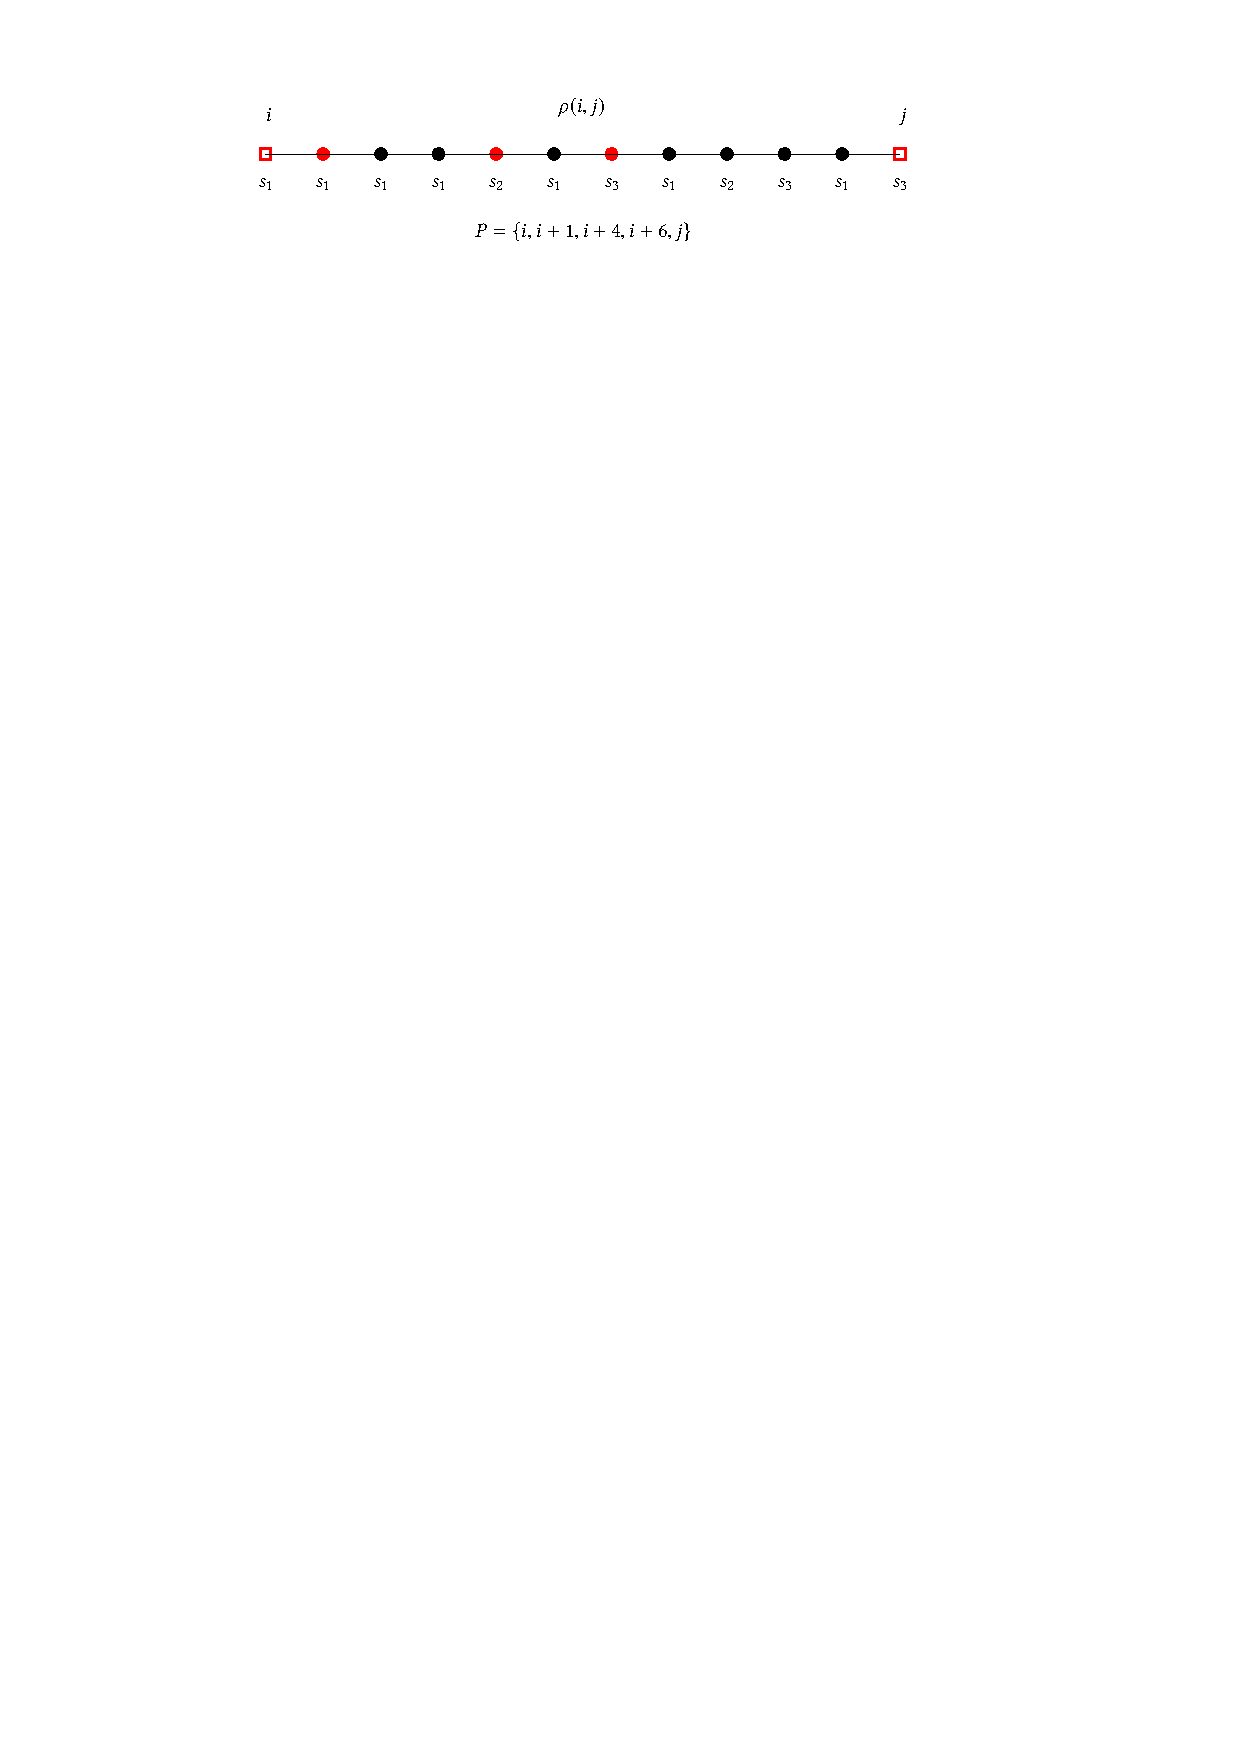
\includegraphics{Chaps/TCS17/prefsampl}}
    \caption{The set $P$ is the prefix-skeleton sampling of $\rho(i,j)=s_1^4s_2s_1s_3s_1\allowbreak s_2s_3s_1s_3$.}
    \label{fig:pref}
\end{figure}
\end{example}

From Definition \ref{def:skeleton}, it immediately follows that the prefix-skeleton sampling $P$ of (any) trace $\rho$ in $[i,j]$ is such that $|P|\leq |\States|+2$, and if $i<j$, then $i+1\in P$.

\begin{definition}[$h$-prefix sampling] \label{def:hprefixsampling}
 Let $\rho$ be a trace of $\Ku$. For each $h\geq 1$, the \emph{$h$-prefix sampling of $\rho$} is the \emph{minimal} set $P_h$ of $\rho$-positions inductively satisfying the following conditions:
\begin{itemize}
  \item for $h=1$: $P_1$ is the prefix-skeleton sampling of $\rho$ in $[1,|\rho|]$;
  \item for $h>1$:
  $(i)$  $P_h\supseteq P_{h-1}$ and
  $(ii)$ for all pairs of consecutive positions $i,j\in P_{h-1}$,
  the prefix-skeleton sampling of $\rho$ in $[i,j]$ belongs to $P_h$.
\end{itemize}
\end{definition}

The following upper bound to the cardinality of prefix samplings easily follows from Definition \ref{def:hprefixsampling}.

\begin{property}\label{property:prefSamBound}
Let $h\geq 1$ and $\rho$ be a trace of  $\Ku$. The $h$-prefix sampling $P_h$ of $\rho$ is such that $|P_h|\leq (|\States|+2)^{h}$.
\end{property}

Lemma~\ref{lemma:prefixSamplingTwo} and Theorem ~\ref{theorem:singleExpTrackModel} below show how to derive, from any trace $\rho$ of the given finite Kripke structure $\Ku$, another trace $\rho'$, induced by $\rho$ and $h$-prefix  bisimilar to $\rho$, such that $|\rho'|\leq (|\States|+2)^{h+2}$. By Proposition~\ref{prop:fulfillmentPreservingSuffixPrefix}, $\rho'$ is indistinguishable from $\rho$ with respect to the satisfiability of any $\AAbarBBbarEbar$ formula $\psi$ with $\nestb(\psi)\leq h$.

In order to build $\rho'$, we first compute the $(h+1)$-prefix sampling $P_{h+1}$ of $\rho$. Then, for all the pairs of consecutive $\rho$-positions $i,j\in P_{h+1}$, we consider a trace induced by $\rho(i,j)$, with no repeated occurrences of any state, except at most the first and last ones (hence, it is not longer than $|\States|+2$). The trace $\rho'$ is just the ordered concatenation (by means of the $\star$-concatenation operator) of all these traces.
The aforementioned bound on $|\rho'|$ holds as, by Property~\ref{property:prefSamBound}, $|P_{h+1}|\leq (|\States|+2)^{h+1}$.
Lemma~\ref{lemma:prefixSamplingTwo} states that $\rho$ and $\rho'$ are indeed $h$-prefix bisimilar.
The proof of such lemma exploits the following technical result (proved in Appendix~\ref{proof:lemma:prefixSamplingOne}).

\begin{lemma}\label{lemma:prefixSamplingOne} Let $h\geq 1$, $\rho$ be a trace of $\Ku$, and let $i,j$ be two consecutive $\rho$-positions in the $h$-prefix sampling of $\rho$.
Then, for all $\rho$-positions $n,n'\in [i+1,j]$ such that $\rho(n)=\rho(n')$, it holds that $\rho(1,n)$ and $\rho(1,n')$ are $(h-1)$-prefix bisimilar.
\end{lemma}

\begin{lemma}\label{lemma:prefixSamplingTwo} Let $h\geq 1$, $\rho$ be a trace of $\Ku$, and $\rho'=\rho(i_1)\rho(i_2)\cdots \rho(i_k)$ be a trace induced by $\rho$, where $1= i_1<i_2 <\ldots < i_k=|\rho|$ and $P_{h+1} \subseteq\{i_1,\ldots,i_k\}$, with $P_{h+1}$ the \mbox{$(h+1)$-prefix} sampling of $\rho$.
Then for all $j\!\in\! [1,k]$, $\rho'(1,j)$ and $\rho(1,i_j)$ are \mbox{$h$-prefix} bisimilar.
\end{lemma}
Note that, as a straightforward consequence, $\rho$ and $\rho'$ are $h$-prefix bisimilar.
\begin{proof}
Let $Q=\{i_1,\ldots,i_k\}$ (hence $P_{h+1}\subseteq Q$) and
%and $P_h$ be the $h$-prefix sampling of $\rho$. By hypothesis $P_h\subseteq Q$.
let $j\in [1,k]$. We prove by induction on $j$ that  $\rho'(1,j)$ and $\rho(1,i_j)$ are $h$-prefix bisimilar. As for the base case ($j=1$), the result holds, since $i_1=1$.

Let us assume that $j>1$. We first show that $\rho(1,i_j)$ and $\rho'(1,j)$ are $0$-prefix bisimilar. Clearly, $\rho(1)=\rho(i_1)=\rho'(1)$, $\rho(i_j)=\rho'(j)$, and $\states(\rho'(1,j))\subseteq\states(\rho(1,i_j))$. Now, if, by contradiction, there was a state $s$ such that $s\in\states(\rho(1,i_j))\setminus \states(\rho'(1,j))$, then for all $l\in Q$, with $l\leq i_j$, $\rho(l)\neq s$. However, the prefix-skeleton sampling $P_1$ of $\rho$ in $[1,|\rho|]$ is contained in $Q$, and the minimal $\rho$-position $l'$ such that $\rho(l')=s$ belongs to $P_1$. Since $s\in\states(\rho(1,i_j))$, we have $l'\leq i_j$ and we get a contradiction, implying that $\states(\rho'(1,j)) = \states(\rho(1,i_j))$.

It remains to prove that:
\begin{enumerate}
  \item for each proper prefix $\nu'$ of $\rho'(1,j)$, there exists a proper prefix $\nu$ of $\rho(1,i_j)$  such that $\nu$ and $\nu'$ are $(h-1)$-prefix bisimilar, and
  \item for each proper prefix $\nu$ of $\rho(1,i_j)$, there exists a proper prefix  $\nu'$ of $\rho'(1,j)$ such that $\nu$ and $\nu'$ are $(h-1)$-prefix bisimilar.
\end{enumerate}

As for (1.), let $\nu'$ be a proper prefix of $\rho'(1,j)$. Hence, there exists $m\in [1,j-1]$ such that
$\nu'=\rho'(1,m)$. By the inductive hypothesis, $\rho'(1,m)$ and $\rho(1,i_m)$ are $h$-prefix bisimilar, and thus $(h-1)$-prefix bisimilar as well by Property~\ref{property:bisimDown}.
%in Section~\ref{sec:bisimilarity}). 
Since $\rho(1,i_m)$ is a proper prefix of $\rho(1,i_j)$, by choosing $\nu=\rho(1,i_m)$, (1.) follows.

As for (2.), assume that $\nu$ is a proper prefix of $\rho(1,i_j)$. Therefore, there exists $n\in [1,i_j-1]$ such that $\nu= \rho(1,n)$. We distinguish two cases:
%
\begin{itemize}
  \item $n\in P_{h+1}$. Since $n<i_j$, there exists $m\in [1,j-1]$ such that $n=i_m$. By the inductive hypothesis, $\rho(1,n)$ and $\rho'(1,m)$ are $h$-prefix bisimilar, and thus $(h-1)$-prefix bisimilar as well by Property~\ref{property:bisimDown}.
  %in Section~\ref{sec:bisimilarity}).
  Since $\rho'(1,m)$ is a proper prefix of $\rho'(1,j)$, by choosing $\nu'=\rho'(1,m)$, (2.) follows.
  \item $n\notin P_{h+1}$. It follows that there exist two consecutive positions $i'$ and $j'$ in $P_{h+1}$, with $i'<j'$, such that $n\in [i'+1,j'-1]$. By definition of $(h+1)$-prefix sampling, there exist two consecutive positions $i''$ and $j''$ in the $h$-prefix sampling of $\rho$, with $i''<j''$, such that $i'$ and $j'$ are two consecutive positions in the prefix-skeleton sampling of $\rho$ in the interval $[i'',j'']$.

  First, we observe that $i'\neq i''$ (otherwise, $j'=i'+1$, which contradicts the fact that $[i'+1,j'-1]\neq \emptyset$, as $n\in [i'+1,j'-1]$). Thus, by definition of prefix-skeleton sampling applied to $\rho$ in $[i'',j'']$, and since $n\in [i'+1,j'-1]$, there must be $\ell\in [i''+1,i']$ such that $\rho(\ell)=\rho(n)$ and $\ell$ is in the prefix-skeleton sampling of $\rho$ in $[i'',j'']$. Hence, $\ell\in P_{h+1}$ by definition of $(h+1)$-prefix sampling. As a consequence, since $\ell<n<i_j$, there exists $m\in [1,j-1]$ such that $\ell=i_m$. By applying Lemma~\ref{lemma:prefixSamplingOne}, we deduce that $\rho(1,n)$ and $\rho(1,i_m)$ are $(h-1)$-prefix bisimilar. Moreover, by the inductive hypothesis, $\rho(1,i_m)$ and $\rho'(1,m)$ are $(h-1)$-prefix bisimilar. Thus, by choosing $\nu'=\rho'(1,m)$, $\nu'$ is a proper prefix of $\rho'(1,j)$ which is $(h-1)$-prefix bisimilar to $\nu=\rho(1,n)$.
\end{itemize}
%
This concludes the proof of Lemma~\ref{lemma:prefixSamplingTwo}.
\end{proof}

We are now ready to prove the exponential small-model property.
%
\begin{theorem}[Exponential small-model property for $\AAbarBBbarEbar$]\label{theorem:singleExpTrackModel}
Let $\rho$ be a trace of a finite Kripke structure $\Ku$ and let $h\geq 0$.
Then there exists a trace $\rho'$ induced by $\rho$, whose length is at most $(|\States|+2)^{h+2}$, such that for every $\AAbarBBbarEbar$ formula $\psi$  with $\nestb(\psi)\leq h$, it holds 
\[\Ku,\rho\models \psi\iff \Ku,\rho'\models \psi.\]
\end{theorem}
\begin{proof} Let $P_{h+1}$ be the $(h+1)$-prefix sampling of $\rho$. For all pairs of consecutive $\rho$-positions $i$ and $j$ in $P_{h+1}$,
%, with $i<j$,
there exists a trace induced by $\rho(i,j)$, whose length is at most $|\States|+2$, featuring no repeated occurrences of any internal state.
We now define $\rho'$ as the trace of $\Ku$ obtained by an ordered concatenation of all these induced traces by means of the $\star$-concatenation operator.
It is immediate to see that $\rho'=\rho(i_1)\rho(i_2)\cdots \rho(i_k)$, for some indexes $1= i_1<i_2 <\ldots < i_k=|\rho|$, where
$\{i_1,\ldots,i_k\}$ contains the $(h+1)$-prefix sampling $P_{h+1}$ of $\rho$. It holds that $|\rho'|\leq |P_{h+1}|\cdot (|\States|+2)$ and since, by Property~\ref{property:prefSamBound}, $|P_{h+1}|\leq (|\States|+2)^{h+1}$, we obtain that $|\rho'|\leq (|\States|+2)^{h+2}$. Moreover, by Lemma~\ref{lemma:prefixSamplingTwo}, $\rho$ and $\rho'$ are $h$-prefix bisimilar. By Proposition~\ref{prop:fulfillmentPreservingSuffixPrefix} the thesis follows.
\end{proof}

Theorem \ref{theorem:singleExpTrackModel} allows us to easily devise an \EXPSPACE\ MC algorithm for $\AAbarBBbarEbar$ formulas (and symmetrically for $\AAbarEBbarEbar$ formulas), which can be obtained from Algorithms \ref{ModCheck2} and \ref{Chk2} by adapting the bounds on the length of considered traces.

We observe that the polynomial small-model property for $\AAbarBBbar$/$\AAbarEEbar$ of the previous section depends \emph{on the specific formula $\varphi$} we are considering (as the input of the MC problem), whereas the exponential small-model property for $\AAbarBBbarEbar$/$\AAbarEBbarEbar$ states the existence of a shorter trace $\rho'$ equivalent to (a generic) $\rho$ with respect to \emph{all} formulas up to a given B/E-nesting depth $h$. As a matter of fact, the former relies on the witness positions, which are defined on $\varphi$; the latter on $h$-prefix/suffix bisimilarity and $h$-prefix/suffix samplings, that are independent of any formula (they are only based on $h$, i.e., the maximum B/E-nesting depth of formulas we want to consider).
%
Therefore, we can say that the latter small-model states a stronger property; however, this \emph{may} lead to a bound on the length of equivalent traces higher than necessary: 
%
we have proved the MC problem for $\AAbarBBbarEbar$/$\AAbarEBbarEbar$ to be in \EXPSPACE, but it is only known to be \PSPACE-hard (since $\Ebar$ or $\Bbar$ are enough for \PSPACE-hardness, as shown in Appendix~\ref{sect:BbarHard}). We do not know whether this  complexity gap is due to the small-model proving a loose bound (that might be strengthened by finding another characterization depending on the input formula as well), or to a weak complexity lower-bound (here, exploiting the other modalities $\A$, $\Abar$ and $\B$/$\E$, along with $\Bbar$ and $\Ebar$ jointly, may enable us to prove a stronger one), or to both at the same time. We will come back to $\AAbarBBbarEbar$/$\AAbarEBbarEbar$ in Chapter~\ref{chap:Gand17}, where we will relax homogeneity and will be able to decrease the complexity upper bound (yet still not matching the lower) also for the  homogeneous case.